 \documentclass{article}

\usepackage{arxiv}

\usepackage[utf8]{inputenc} % allow utf-8 input
\usepackage[T1]{fontenc}    % use 8-bit T1 fonts
\usepackage{hyperref}       % hyperlinks
\usepackage{url}            % simple URL typesetting
\usepackage{booktabs}       % professional-quality tables
\usepackage{amsfonts}       % blackboard math symbols
\usepackage{nicefrac}       % compact symbols for 1/2, etc.
\usepackage{microtype}      % microtypography
\usepackage{lipsum}
\usepackage{graphicx}
\usepackage{titlesec}
 \usepackage{mathtools}
\graphicspath{ {../figures/} }

\renewcommand\vec{\mathbf}
\titleformat{\section}
{\normalfont\LARGE\centering\bfseries}{}{0em}{}

\titleformat{\subsection}
{\normalfont\Large\bfseries}{}{0em}{}

\title{ Generating Hierarchy in Hollywood according to consumer preferences }

\author{
 Marlin Figgins \\
  University of Washington \\
  \texttt{mfiggins@uw.edu} \\
   \And
 Xingzi Xu \\
  Stanford University \\
  \texttt{xingzix@stanford.edu} \\
  \AND
 Shashank Dalmia \\
  University of California Berkeley\\
  \texttt{shashankdalmia24@berkeley.edu} \\
  \And
 Aditya Nair \\
  University of California Berkeley\\
  \texttt{adityanair@berkeley.edu} \\
}

\begin{document}
\maketitle
\begin{abstract}
Hollywood and the larger film industry is highly profitable and commercial films have been embedded in American culture, but Hollywood still to some extent maintains it own unique culture. Though Americans spend millions and millions of dollars annually on this industry, it can be difficult to ascertain the extent to which film viewers influence the future and culture of the industry itself. To begin approaching this, we ask, "To what extent do consumer preferences and evaluations affect the social network of director-actor collaborations in Hollywood?".\\

In order to take advantage of the relationships between both actors and directors, we develop a social network describing the collaborations between various actors and directors. We identify various factors statistically associated with the probability of directors and actors collaborating with one another, then using a network dynamic model to infer which factors determine hierarchy between actors and directors. This allows us to determine a ranking of individuals in Hollywood, which we determine to be dominated primarily by actors. Further, analysis shows that Academy Awards carry significant weight in determining one's future collaborators, but additionally that one's future collaborators are likely to be similarly rated to oneself according to community ratings metrics on online communities like IMDb. This suggests that though prestigious awards like the Oscars awards can carry weight in determining one's career trajectory, it can prove to be difficult to climb the social ladder in Hollywood without being well-received by consumers.
\end{abstract}

\newpage % Start Technical summary on new page.

\section{Technical Summary}

\subsection{Data exploration.}
In order to explore the relationship between consumer preferences and directors/actors and to potentially predict the prestige of a director/actor based on these preferences, we use the \texttt{movie\_industry} and \texttt{the\_oscar\_award} data sets. The first data set contains relevant information of the most popular movies (approximately 220) in each year from 1986 to 2016 such as each film's \texttt{director} and its \texttt{star}, which we use to extract information about collaborations between directors and actors. We also use columns including \texttt{gross}, \texttt{genre}, \texttt{rating}, \texttt{score}, and \texttt{votes} to learn more information of each director and star. The latter data set contains Oscar Awards nominations and wins beginning in 1927, which we use as a proxy for measuring prestige and/or success. Since the data set is the full list of Oscar Awards nominations across all categories, we narrow our focus to the subset of the data which features actor, actress, and directing awards. 

From exploratory data analysis on \texttt{movie\_industry}, we note that category features such as \texttt{genre} and \texttt{rating} have levels with very small samples, which needs further bucketing for one-hot encoding. It is also interesting to see positive correlations between score and number of votes as well as score and gross of the movie. The variance of score is big for movies with small number of votes, yet once a movie has more than $\sim$750,000 votes, its score is very high. With time series analysis, we find that \texttt{budget}, \texttt{gross}, \texttt{score}, and \texttt{votes} all increase over time except a big drop for number of votes in 2015. The increasing gross might be a result of inflation. However, since we are interested in the interactions between directors and actors on a yearly basis, inflation would not present a big impact in our context.

The data cleaning process involves cleaning of the strings in \texttt{the\_oscar\_award}, especially in the \texttt{category} and \texttt{name} variables. We cross check the names in \texttt{the\_oscar\_award} and \texttt{movie\_industry} and make sure that the same individual has exactly the same name strings in both data sets. We also re-encode \texttt{rating} in  \texttt{movie\_industry} to unify "UNRATED", "NOT RATED", and "Not specified". After initial data cleaning and filtering out nominations of movies before 1986, we have 852 nomination entries with 171 wins. Of directors and stars represented in \texttt{movie\_industry}, 12.5\% have been nominated for an Oscar. 

We also note some limitations of our data sets. First, we only have around 220 movie records per year in the \texttt{movie\_industry}. There are 82 nominees which are represented in \texttt{the\_oscar\_award} which are not represented in \texttt{movie\_industry}. Second, \texttt{movie\_industry} data set only features one star for each movie, either the leading actor or the leading actress, and therefore, we are limited in our ability to capture the relationship between directors and supporting actors.

\subsection{Determining covariates.}

In order to determine how a network of director-actor collaborations evolves, we attempt to discern what features in our data likely influence the probability of future collaborations. We conduct a series of hypothesis tests with the continuous features and categorical features in \texttt{movie\_industry} as well as counts of Oscar nominations and wins in order to check whether they have significantly different distributions for director-actor pairs which have or have not collaborated.  

There are 6,908,536 possible combinations of director-actor combinations in total, out of which 6,306 director-actor pairs have collaboration histories. Accordingly, the data is divided into two parts: pairs that have worked together and pairs that have not. Our objective is to determine features that help distinguish director-actor pairs that have worked together versus those who haven't for assessing the likelihood of a collaboration in the future.


 We have three expectations and calculate the statistics correspondingly as followed:

\begin{enumerate}
\item  A pair is more likely to work together if they have similar number of \texttt{votes}/\texttt{score}/\texttt{gross}. 
\begin{itemize}
    \item Absolute difference of the log of total gross for a director and the log of total gross for an actor.
    \item Absolute difference of the log of mean votes for a director and the log of mean votes for an actor.
    \item Absolute difference of the log of mean score for a director and the log of mean score for an actor.
\end{itemize}

\item  A pair is more likely to work together if they have similar number of Oscar nominations and wins.
\begin{itemize}
    \item Absolute difference of total nominations for a director and total nominations for an actor.
    \item Absolute difference of total wins for a director and total wins for an actor.
\end{itemize}

\item  A pair is more likely to work together if they have both worked in movies of similar \texttt{genres} and \texttt{ratings}. 
 \begin{itemize}   
    \item Total Variation Distance between proportion of movies in each genre. (We only calculated values for the top 8 genres which made up ~98\% of the data set.)
    \item Total Variation Distance between proportion of movies in each rating category. (We only calculated values for the top 5 rating categories which made up ~99\% of the data set.)
\end{itemize}
\end{enumerate}

Therefore, for each director-actor pair, we calculate the difference between the pair, visualize and compare the distribution of the difference between the collaboration group and non-collaboration group, and calculate the $p$-values under T-Test and Kolmogorov-Smirnov Test. The null hypothesis is that there is no significant difference between the two groups. Figure \ref{fig:t-test-fig} shows features that we identified that are statistically significant in inferring whether a director-actor are likely to work together. We could see that from the result, the distributions of collaboration group are very different from those of the non-collaboration group and the $p$-values are all very small, pointing towards the alternative. Through this, we can identify significant covariates for further modeling. 

\begin{figure}
    \centering
    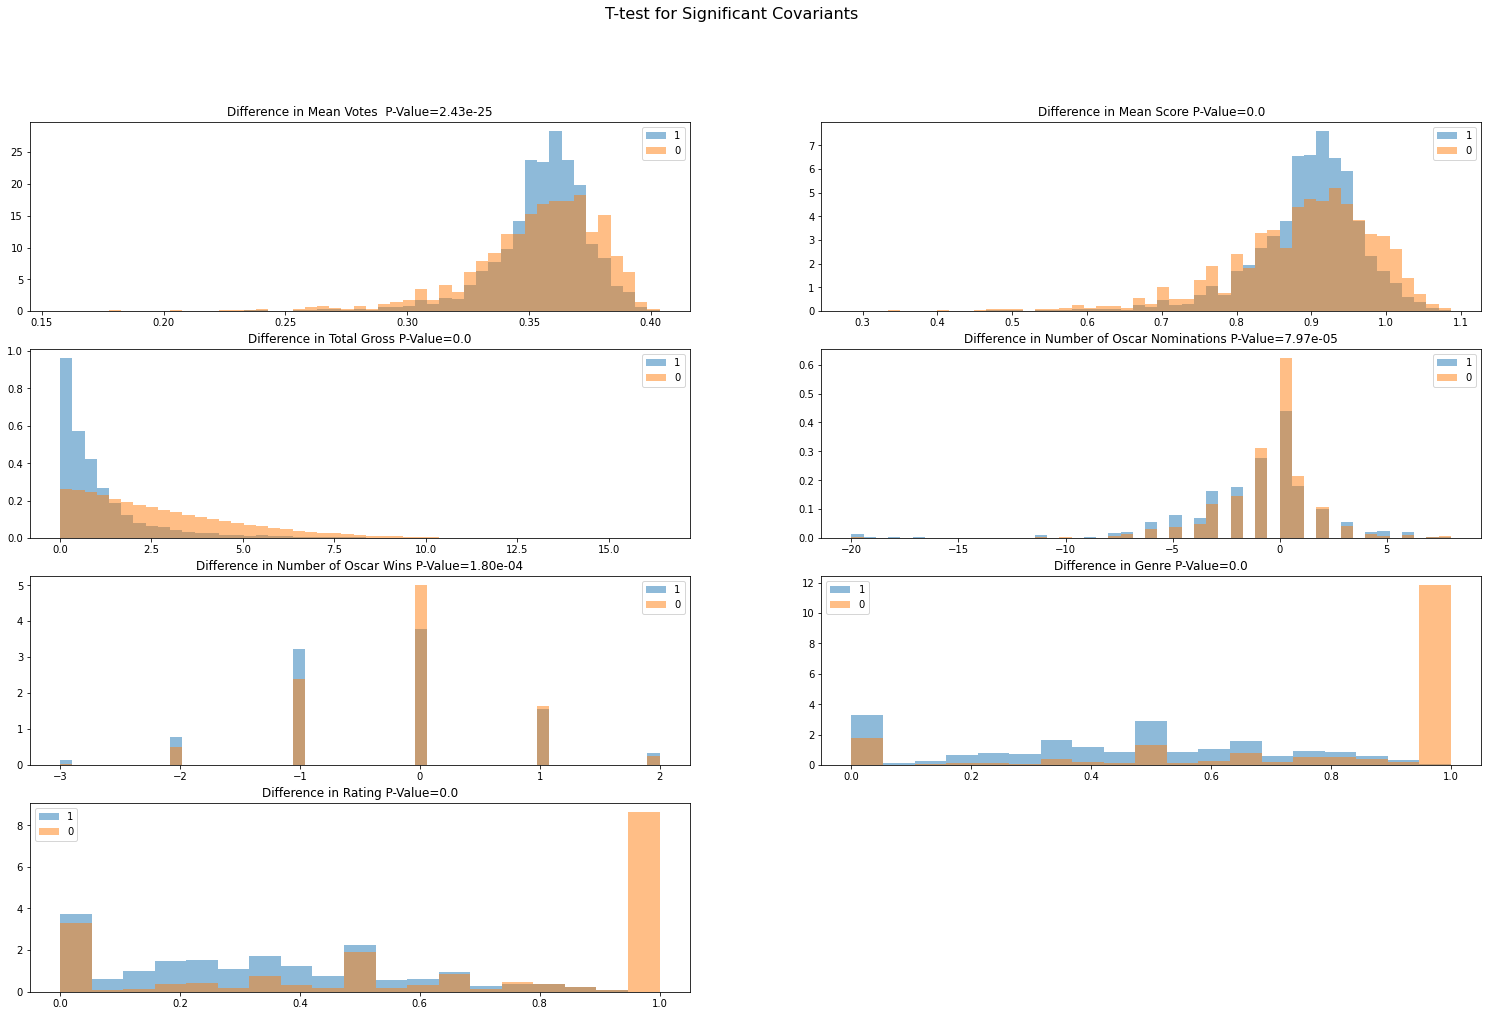
\includegraphics[scale=0.35]{T-test_for_Significant_Covariants.png}
    \caption{Difference in Distributions for Significant Covariates. Blue corresponds to individuals who have worked together. Orange corresponds to those who have not.}
    \label{fig:t-test-fig}
\end{figure}

\bigskip
\begin{table}
  \centering
\begin{tabular}{ |p{7cm}||p{4cm}|p{4cm}| }

 \hline
 \multicolumn{3}{|c|}{$p$-values of significant covariates under T-test and Kolmogorov-Smirnov Test} \\
 \hline
        & T-Test & Kolmogorov-Smirnov Test \\
 \hline
Mean Votes &  6.09e-17     &  9.08e-56  \\
Mean Score  &  3.19e-13   &   7.48e-56   \\
Total Gross &  0.0   &  0.0   \\
Nominations &  2.05e-09   & 9.51e-10    \\
Wins &  8.33e-09   & 2.11e-07   \\
Genre &  0.0  & 0.0   \\
Rating & 0.0  & 0.0   \\
 \hline
\end{tabular} 
\newline\newline
  \caption{$p$-values of significant covariates under T-test and Kolmogorov-Smirnov Test}\label{tab1}
\end{table}


\subsection{Generating covariates.}

%TODO: looks abrupt
There are 2759 unique directors and 2504 unique actors across the 31 years of the movie industry data set. There are 171 people in the data set who have worked as both an actor as director and thus feature in both actor and director categories . For our analysis we consider them separately. Therefore, the covariates for "Clint Eastwood" as an actor and director are calculated separately. We will refer to these unique actors and directors as agents from here on. We calculate the covariates at every time step. Thus the granularity of our data set is every agent at a particular time step. There are a total of 163,153 observations (31 time steps $\times$ 5263 agents). For each observation, we calculate 18 features which we believe to be covariates. They are as follows:

\begin{itemize}
  \item \texttt{log\_total\_gross} : calculated as $\ln$(total gross+1) of all movies of the particular agent until that time step.
  \item \texttt{mean\_score} : mean votes calculated as the mean of scores of all movies of the particular agent until that time step; 0 if no movie done until that time step.
  \item \texttt{mean\_votes} : mean votes calculated as the mean of votes received of all movies of the particular agent until that time step; 0 if no movie done until that time step.
  \item \texttt{Comedy}, \texttt{Drama}, \texttt{Action}, \texttt{Crime}, \texttt{Adventure}, \texttt{Biography}, \texttt{Horror}, and \texttt{Animation} : Number of movies under each of those genre categories for each agent until that time step.Note that there are more genre classifications in the movie industry data set. However, these genres make up ~98\% of the data set. To reduce complexity, we do not create covariates for the remaining categories.
  \item \texttt{R}, \texttt{PG-13}, \texttt{PG}, \texttt{NOT RATED}, and \texttt{G} : Number of movies under each of those rating categories for each agent until that time step. 'Not specified', 'UNRATED' and 'NOT RATED' rating categories in the movie industry data set have been reclassified as 'NOT RATED'. Note that there are more rating classifications in \texttt{movie\_industry}. However, the aforementioned categories make up approximately 99.6\% of the data set. To reduce complexity, we do not include remaining categories as covariates.
  \item \texttt{nominations} and \texttt{win\_counts} : Number of Oscar nominations and wins of the particular agent until that time step.
  
\end{itemize}

\subsection{Director-actor collaboration networks.}

\begin{figure}
    \centering
    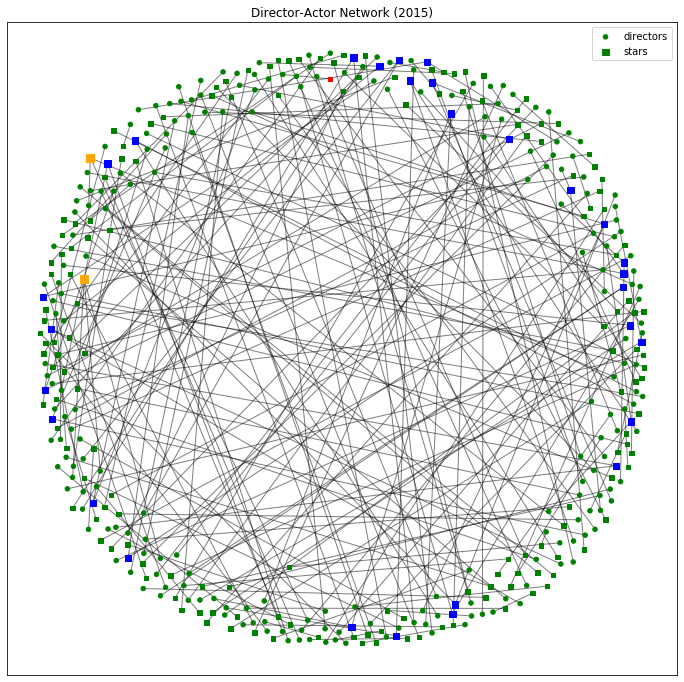
\includegraphics[scale=0.35]{Director_Actor_Network_2015.png}
    \caption{A densely populated graph with node colors delineating how active the corresponding agent is. Green, blue and yellow represent the agent working on 1, 2, and 3 movies respectively. Leonardo DiCaprio is highlighted in red for your viewing pleasure.}
    %TODO: Explain how the coloring is working here.
    \label{fig:t-graph-fig}
\end{figure}

% Graph 
\begin{figure}
    \centering
    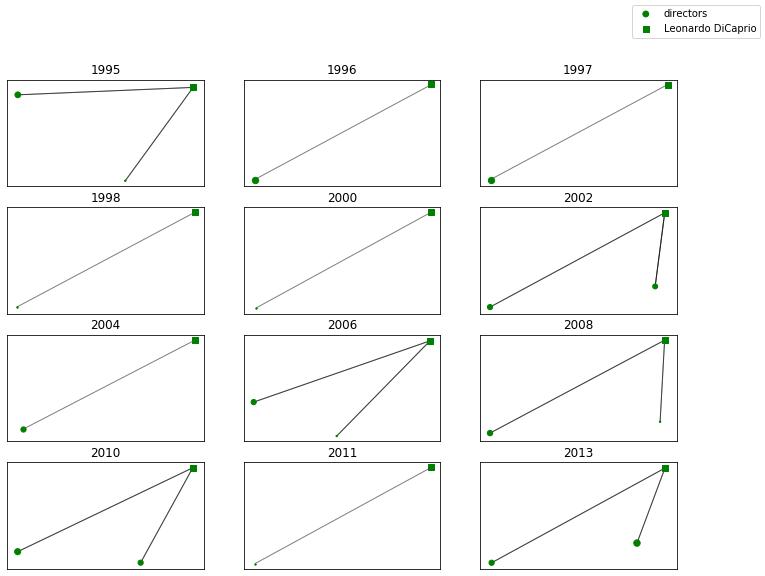
\includegraphics[scale=0.5]{DiCaprio_Longitudinal_Network_2.png}
    \caption{A longitudinal analysis of everyone's favorite actor, Leonardo DiCaprio, with node size scaled by the log of the total gross. Note that though he becomes increasingly successful, he often works with directors who make nowhere near as much as he does}
    %TODO: Explain how the coloring is working here.
    \label{fig:t-graph-fig-2}
\end{figure}
%TODO: Add color coding of graph

\paragraph{Choosing to use a graph.}
For our director-actor collaboration networks, we find a model that integrates well with the rest of our pipeline and will be easy to transfer after creation and storage so our team can interact with the model on their own time. Logically, we decide on using a graph structure, which will be bipartite by nature of the restrictions we placed on the definition of collaboration, that can be easily transferred using some representation of an adjacency matrix. 
% break the above into shorter lines to make clearer

% explain the indexing of delta t
\paragraph{Creating the model.}
Mechanically, we iterate through \texttt{movie\_industry} for every year \emph{t}, isolate all director-actor relationships from that year, and begin constructing a network by connecting the director and actor present in each relationship. For each actor and director pair present in the \texttt{movie\_industry} data set, we need to represent a way to represent their collaboration or lack thereof. Mathematically, we present the complete network as a set $\{\Delta(t)\}$ indexed by the year. Each element $\Delta(t)$ is a square matrix with elements

\begin{equation}
    \Delta_{ij}(t) = \begin{cases} 1 & \text{if agents $i$ and $j$ have collaborated in year $t$,}\\
    0 & \text{ otherwise.}
    \end{cases}
\end{equation}
%The Graph class we create for this purpose also supports selecting a subset of years to reduce computation time even further.
 Loading the graph into a visualization also allows us to see some interesting relationships between groups of agent pairs. For example, in Figure \ref{fig:t-graph-fig}, we see that actors that work on multiple movies in a year work with smaller directors. In Figure \ref{fig:t-graph-fig-2}, we can see DiCaprio's evolution over time (taking the log of total gross stops his node from blotting out the entire graph, but makes it quite difficult to see how successful his colleagues are)
 
 %TODO: Notice that directors tend to work on a single film. Maybe rephrase this statement 2? Directors rarely get to work on more than one popular film a year. Actors can in few cases work on more than one popular fil,s.

\paragraph{Computational Burden.}
With over 5000 unique agents, constructing and storing these as networks as adjacency matrices yielded extremely large files . To assuage this, we stored the matrices in a sparse matrix format, which brought the full storage cost down by 99.7\%. We realized this would be possible because our graph is bipartite in nature (directors are connected only to actors and vice versa), so two quadrants of the adjacency matrix are entirely filled with zeros.

%TODO: Be sure to use the notation $\Delta(t)$ for the graph of collaborations at time $t$.
\subsection{Modeling hierarchy in Hollywood collaborations.}

In order to understand how consumer preferences contribute to the formation of hierarchy. We rely on a network dynamics model. This formulation has been used to recreate hierarchies in higher education such as those governing prestige in PhD-granting institutions in mathematics. \cite{Kawakatsu2020}.

\paragraph{Collaboration dynamics.} We take in various covariates which affect individual actors' and directors' probability of working with another in a particular year as a matrix $\vec{X}$ with each column $\vec{x}_1, \ldots, \vec{x}_k$ corresponding to different predictors. The matrix $X$ contains director-actor specific information so that $x_{im}$ is the value of the $m$-th covariate corresponding to the $i$-th agent. Then we determine the utility of a collaboration between agents $i$ and $j$ as 

\begin{equation}
    u_{ij} = \sum_{m = 1}^{k} \beta_m \left| x_{im} - x_{jm}\right|.
\end{equation}

In this way, estimating the coefficient vector $\vec{\beta} = (\beta_1, \beta_2, \ldots, \beta_k)$ acts as a way to compute relative weight of how differences in each factor contribute to predicting collaborations between individuals. 

We then compute the probability of a collaboration occurring between individuals $i$ and $j$ in that year as 
\begin{equation}
    p_{ij} = \frac{e^{u_{ij}}}{\sum_{k = 1}^{n} e^{u_{ik}}}.
\end{equation}

\paragraph{Computing Hierarchy.}

Using the probabilities described above, we are able to compute the rankings of various individuals in terms of how likely it is for others to work with them. Therefore, we compute the rank of individual $i$ as 

\begin{equation}
    \gamma_i = \sum_{j=1}^{n} p_{ij}.
\end{equation}

\paragraph{Inference.}

Given our generated director-actor collaboration network $\{\Delta(t)\}$, we can compute the maximal likelihood estimates of $\vec{\beta}$ associated with our model. The likelihood for the parameters $\vec{\beta}$ is given implicitly through
\begin{equation}
    \mathcal{L}(\vec{\beta} \mid \{\Delta(t)\}) = \sum_{i,j,t} \Delta_{ij}(t) \log p_{ij}(t) + C
\end{equation}

    where $C$ is a constant which does not depend on $\vec{\beta}$. 

We use this framework to generate hierarchies within our director-actor network. Our goal is to infer the maximum likelihood coefficient vector $\hat{\beta}$. We take advantage of the fact that this problem is convex in $\vec{\beta}$ and solve for $\vec{\beta}$ using convex optimization schemes implemented in SciPy \cite{SciPy2020}. This alongside our computation of rank allows us to infer which factors affect the probability of an actor becoming well-connected.

\begin{table}
\centering
\begin{tabular}{lcc}
\toprule
                 & Small Model &  Full Model \\
\midrule
 log\_total\_gross &   -7.41e-03 &   -9.09e-03 \\
      mean\_score &    3.66e-03 &    9.50e-03 \\
      mean\_votes &   -1.12e-07 &   -1.71e-07 \\
          Comedy &             &   -3.78e-03 \\
           Drama &             &    4.93e-02 \\
          Action &             &   -8.45e-03 \\
           Crime &             &   -2.41e-02 \\
       Adventure &             &   -3.32e-02 \\
       Biography &             &    2.39e-02 \\
          Horror &             &   -2.01e-02 \\
       Animation &             &   -1.18e-03 \\
               R &             &    3.05e-03 \\
           PG-13 &             &   -1.07e-03 \\
              PG &             &   -3.45e-02 \\
       NOT RATED &             &   -1.61e-02 \\
               G &             &    3.97e-03 \\
     nominations &             &    5.99e-02 \\
      win\_counts &             &    1.07e-02 \\
\bottomrule
\end{tabular}
\caption{Inferred weights $\hat{\beta}$  corresponding to variables above. Larger, positive parameters indicate preference for collaborations between agents of similar quantities e.g. we see a strong preference for Academy award nominated individuals to collaborate with one another as well as a preference for individuals with similarly consumer-rated filmographys to collaborate.}
\label{table:beta_table}
\end{table}

\paragraph{Implementation.}
%TODO: Mention computational issues with this due to sheer volume of data set. We've been able to reduce the computational load through the usage of sparse arrays and built-in methods for computing with these objects in sklearn and scipy.

Despite having access to covariates available for 31 years, we restrict this hierarchy model to the most recent 10 years of data (2007-2016) for several reasons:

\begin{enumerate}
    \item \textbf{Individual history.} In order to properly account for the fact that some directors and actors begin their careers before the time at which our data begins, we restrict our inference of the hierarchical dynamics to the 10 most recent years, so that we can use the entire history of the agents active in that time period in our analysis.
    \item \textbf{Computational burden.} By restricting the time frame in our analysis, we reduce the computation necessary for a single evaluation of the likelihood by reducing the number of agents active in this time period, which is expensive to evaluate as the number of operations necessary scales $O(n^2)$ with $n$ agents. This issue is partially remedied by representing $\Delta(t)$ as a sparse matrix. 
\end{enumerate}

\begin{figure}
    \centering
    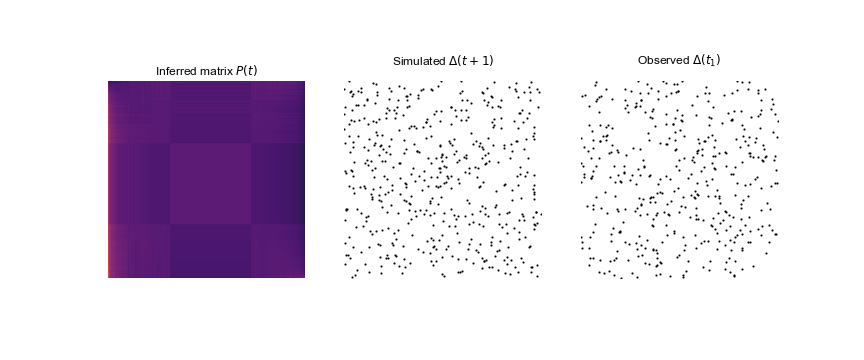
\includegraphics[scale=0.5]{matrix_plot.png}
    \caption{Visualizing the various matrices generated by our model. Using the probability matrix associated with the inferred $\hat{\beta}$, we can simulate hypothetical collaborations among agents in our network which resemble our observed collaboration network.}
    \label{fig:my_label}
\end{figure}

\paragraph{Findings.}

Using the inference scheme described previous, we inferred model parameters describing the relative weight of certain parameters in determining individual connections and thereby hierarchy. These values are presented in table \ref{table:beta_table}. In both models, we can see that the mean score of an individual's past films as evaluated by consumers plays a significant role in determining hierarchy. In other words, individuals are more likely to collaborate with individuals of similar filmography quality as evaluated by consumers. We also see that the parameters corresponding the Academy Award nominations and wins are positive and relatively large indicating a preference for individuals who have been nominated to work with one another.

This inference also allows us to visualize the rankings of individuals. We present that 5 most highly ranked and 5 lowest ranked agents in \ref{fig:top_bottom}. 

\begin{figure}[ht]
    \centering
    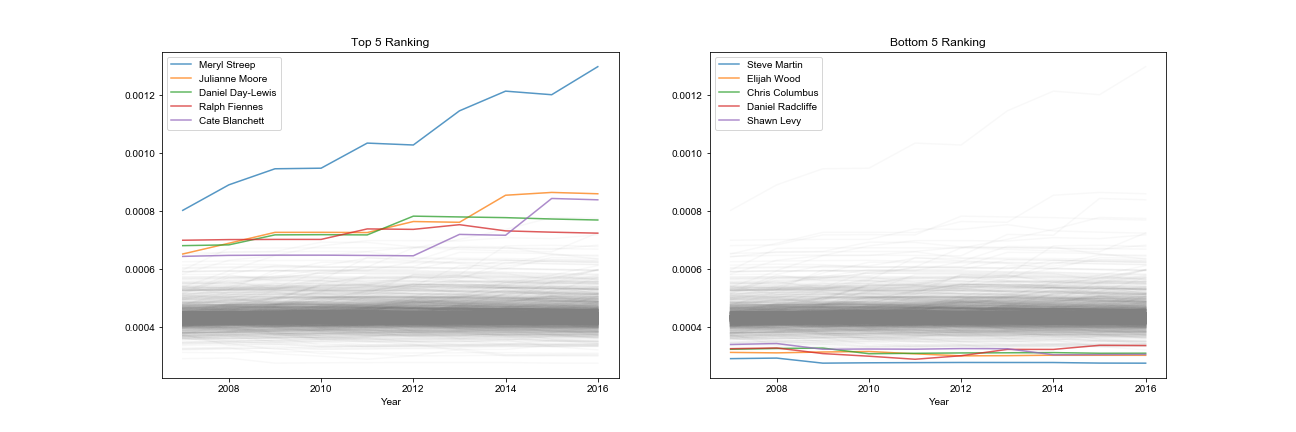
\includegraphics[scale=0.4]{rankings.png}
    \caption{We visualize the top and bottom ranked agents according to our model. 'Top' and 'Bottom' were computed according actors sum total score across the years 2007 to 2016.}
    \label{fig:top_bottom}
\end{figure}

Looking at the rankings here, there appears to be a multitude ways of climbing the hierarchy. One such way is appearing in movies with large commercial success. Other ways is appearing with alongside highly-ranked agents. Alternatively, if you're Meryl Streep, you do it all!  We also see a pattern among the top 5 ranked agents all have been nominated for Academy Awards previously and 4 are winners.

\paragraph{Possible extensions of this method.}

The method described above is extremely extensible. Though, we relied on covariates generated from \texttt{movie\_industry} and \texttt{the\_oscar\_award} for our estimates in \ref{table:beta_table}. This methodology can also be used to infer the importance of network metrics such as node degree, PageRank centrality as well as variables found in other data sets.

Another possible dimension for extension is in the role of various regularization techniques. For example, as regularization using the $L^1$ norm is known to promote sparsity, this method could be similarly expanded for sparse regression on the various covariates to identify features which contribute the most to observed collaboration and hierarchy within the larger network.
\newpage

\bibliography{references}
\bibliographystyle{ieeetr}
\end{document}
